\RequirePackage[T1]{fontenc}
\documentclass[10pt,journal,letterpaper]{IEEEtran}
\usepackage{amsmath,amssymb,amsthm,booktabs,array,microtype}
\usepackage[hidelinks]{hyperref}
\usepackage{fancyhdr,tikz,graphicx}
\usetikzlibrary{arrows.meta}
\hypersetup{pdftitle={Unbounded Viewstamped Replication Revisited for Diskless Strong Consistency},pdfauthor={Simon Massey}}
\newcommand{\paperrevision}{RESEARCH CHECKPOINT --- 11 SEPTEMBER 2026}
\newcommand{\paperversion}{DRAFT}
\IfFileExists{version.tex}{\input{version.tex}}{}
\pagestyle{fancy}
\fancyhf{}
\fancyhead[R]{\footnotesize\thepage}
\fancyfoot[C]{\scriptsize\paperrevision\ --- \paperversion}
\renewcommand{\headrulewidth}{0pt}
\setlength{\emergencystretch}{1em}
\raggedbottom
\newtheorem{theorem}{Theorem}
\newtheorem{lemma}{Lemma}
\newcommand{\QI}{\mathcal{Q}^{\mathrm I}}
\newcommand{\QII}{\mathcal{Q}^{\mathrm {II}}}
\newcommand{\code}[1]{\texttt{#1}}
\title{Unbounded Viewstamped Replication Revisited\\for Diskless Strong Consistency}
\author{Simon Massey\thanks{Author draft. Correspondence: simon.massey@stenographer.cloud.}}
\begin{document}
\maketitle
\thispagestyle{fancy}

\begin{abstract}
Small replicated metadata should not require a disk flush on the critical path.
Unbounded Viewstamped Replication Revisited is a protocol design for embedding
strong consistency with volatile normal-path replication and crash-stop
reincarnation.
A cleanly stopped process restarts with its identity and flushed state.
A crashed process permanently retires its old identity and rejoins under a fresh
identity, obtaining state and voting authority through reconfiguration.
Its organising mechanism is leader overlap: where the leader is the sole
intersection of the active decision quorum and the next prepare quorum, it
withholds its own promise so that preparation can proceed while the active
quorum remains usable.
Five-voter replacement uses six committed batches, including exact doubling
and halving. A constructive Rust solver also computes paths between arbitrary
weighted-majority configurations with an available majority at each endpoint.
The Lean development proves weighted reachability and a phantom-identity
casting-vote construction, alongside agreement and identity exclusion for a
three-voter warm-up and a five-voter replacement. The addendum published
with the code separates the proof contracts and executable checks.
\end{abstract}

\begin{IEEEkeywords}
Crash-stop, leader overlap, reconfiguration, strong consistency, Viewstamped Replication.
\end{IEEEkeywords}

\section{Introduction}\label{sec:intro}
Oki and Liskov introduced Viewstamped Replication in 1988~\cite{vr}.
Liskov and Cowling's 2012 Viewstamped Replication Revisited (VRR) eliminated
disk writes during normal processing and view changes~\cite{vrr}.
Replication therefore retained the state needed for agreement without adding a
local disk flush to each update. The remaining difficulty was how to bring a
replica back after loss of that state.

Michael \emph{et al.} exposed a safety failure in VRR's recovery mechanism in
2016~\cite[Sec.~4.2 and Appendix~A.1]{diskless}.
A replica can send a view-change commitment, crash, and return in an older view
having forgotten the commitment.
It can then help commit an operation that a later leader loses when delayed
view-change messages arrive.
Their counterexample breaks linearizability, including when channels preserve
message order.
The authors provide a virtual stable storage construction to support diskless
crash recovery.
Their result makes the problem precise: restoring a replica's data must also
preserve the commitments made by its identity.

Unbounded Viewstamped Replication Revisited (uVRR) repairs this failure by
making a crash final for the protocol identity.
The crashed identity never resumes execution.
The process that replaces it joins under a fresh identity, receives state from
the cluster, and acquires voting authority through committed membership changes.
Messages sent before the crash remain messages of the old identity; the new
process cannot add fresh votes to that identity's history.
A cleanly stopped process can instead restart under its existing identity because
it has preserved its protocol state.
Startup fencing and clean shutdown use durable writes, keeping those writes
outside normal replication. Loss of volatile state therefore leads to replacement
of a member: crash recovery becomes crash-stop reincarnation.

Turner supplies the construction that connects this lifecycle to continued
replication~\cite{turner}.
Where the leader is the sole intersection of an active decision quorum and the
next prepare quorum, it can withhold its own promise while collecting the others.
The active quorum remains usable during that preparation; the leader completes
the handover with its own local promise.
We use this leader overlap to organise reincarnation.
For three unit-weight voters, replacement takes two committed batches.
For five, the weighted schedule has six, including exact doubling and halving.
The addendum published with the code~\cite{artifact} gives the proof ladder,
a general configuration-path constructor and an abstract casting-vote
completion using fresh identities. Turner's agreement argument supplies the
basis for composing safe adjacent configuration boundaries.

Together, these ideas retain VRR's diskless normal path while giving failed
members a route back through fresh identities.
The intended setting is agreement over small amounts of metadata embedded in a
distributed application~\cite{motivation}.
Such a service can coordinate membership or advisory-lock metadata without
putting synchronous persistence on every update's critical path.
Its normal replication need not wait for a disk flush or batch updates to
amortise one.

Section~\ref{sec:method} develops the lifecycle and leader-overlap construction.
Section~\ref{sec:results} starts with three-voter Crash-Stop-Reincarnation
and extends the argument to five voters, stating the history invariants needed
for agreement, exclusion of the evicted voter and identity nonreuse.
Section~\ref{sec:discussion} develops the metadata applications; the accompanying
addendum gives the mathematical working and verification evidence.
The name ``unbounded'' follows Turner's treatment of pipelining through
reconfiguration: agreement does not depend on a fixed bound on outstanding slots.

\section{Method}\label{sec:method}
\subsection{Processes, state and identity}
The agreement model is asynchronous and non-Byzantine. Messages may be delayed, and an old message retains the identity that issued it. Each incarnation has a logical identity distinct from its physical host. The lifecycle must ensure that an identity never produces new protocol actions after a replacement incarnation takes over.

A clean stop first quiesces protocol processing, then flushes the state required for restart, and finally records a durable stopped marker. On startup, a valid stopped marker permits the process to reload that state and enter \emph{Restarting} with the same identity. Before sending protocol messages it durably records that it is running again. This boot fence prevents a later crash from being mistaken for another clean restart. A restarting process retains its promises and accepted state, so ordinary timeout processing is permitted by the design.

Without a valid clean-stop marker, startup enters \emph{Joining} under a fresh identity. The old identity is crash-stopped. Cached state may reduce transfer work, but it provides no voting authority. The joiner asks the leader to evict the old incarnation and admit the new one; the leader can send missing state while coordinating the change. A joiner does not vote or initiate a view change. Its authority comes from the committed configuration, never from the fact that it shares a host with a former voter.

The implementation design uses replicated superblock markers and majority interpretation of valid marker copies. This paper abstracts that mechanism as correct clean-stop classification and durable identity fencing. The Lean result concerns the resulting lifecycle; it does not model the storage protocol itself.

\subsection{Quorums across eras}
An era determines the quorum families for a suffix of log slots. Write $\QI_e$ for its phase-one family and $\QII_e$ for its phase-two family. The history model requires the following within-era and adjacent-era intersections:
\begin{align}
q\cap r&\ne\varnothing
&& (q\in\QII_e,\ r\in\QI_e),\label{eq:same}\\
q\cap r&\ne\varnothing
&& (q\in\QI_e,\ r\in\QII_{e+1}).\label{eq:adjacent}
\end{align}
The direction in~\eqref{eq:adjacent} matters: the earlier phase-one quorum must meet the later decision quorum. These conditions are part of Turner's era-based agreement argument~\cite{turner}.

Our concrete schedule uses the same strict weighted-majority family for both phases. If $w_e(n)$ is a nonnegative integer weight on a finite support, a quorum $q$ satisfies
\begin{equation}
2\sum_{n\in q}w_e(n)>\sum_n w_e(n).
\label{eq:majority}
\end{equation}
The weighted proof establishes the requisite intersections when successive configurations differ by at most one unit of total absolute weight. Membership records for zero-weight nodes may change in the same batch without altering~\eqref{eq:majority}. A crash itself does not change any weight; only committed configuration commands do.

\subsection{The leader as the overlap}
Suppose a leader $\ell$ uses ballot $b$ with an active decision quorum $q$. To prepare ballot $b'>b$ for the next era, it chooses a prospective phase-one quorum $q'$ with
\begin{equation}
q\in\QII_e,\qquad q'\in\QI_{e+1},\qquad q\cap q'=\{\ell\}.
\label{eq:leader}
\end{equation}
This is Turner's casting-vote condition~\cite{turner}. The leader first sends prepare requests only to $q'\setminus\{\ell\}$. Their promises do not disable an acceptor in $q$. The leader withholds its own promise and may continue proposing at $b$, provided no other event invalidates the old ballot's guards.

After receiving those promises, the leader chooses the suffix boundary $k$ and makes its own promise locally. Phase one is then complete without another network exchange for the leader's response. Proposals at $b'$ must still obey the normal rule for preserving values reported by phase one. Figure~\ref{fig:overlap} shows the message order.

Decision quorums follow the era of the \emph{slot}, not simply the era associated with a ballot. Consequently, continuing to decide later-era slots at $b$ also requires a quorum valid for those slots. In the concrete pivot below, the active quorum is a majority in both adjoining eras.

\begin{figure*}[t]
\centering
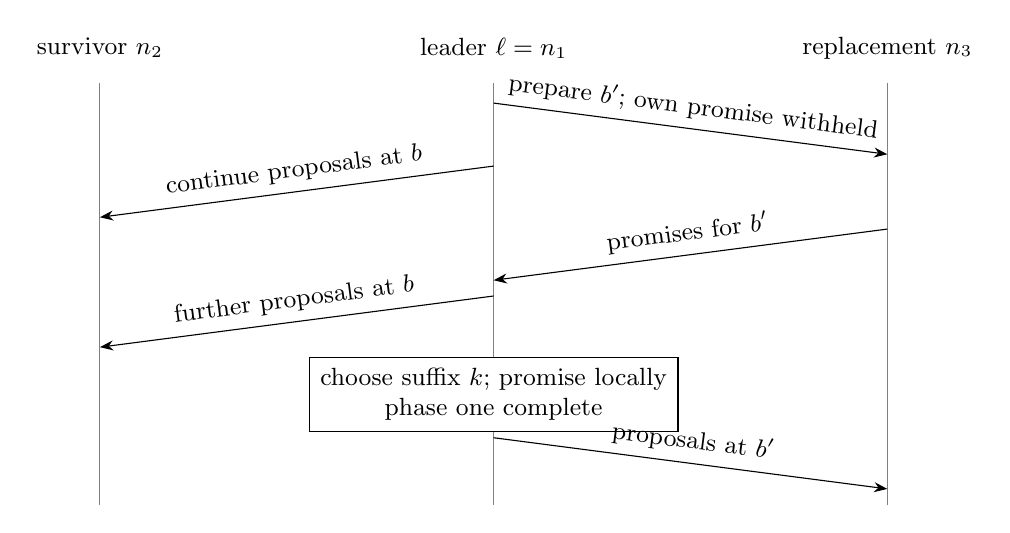
\begin{tikzpicture}[x=1cm,y=1cm,>=Stealth,font=\small]
\node at (0,0.45) {survivor $n_2$};
\node at (5,0.45) {leader $\ell=n_1$};
\node at (10,0.45) {replacement $n_3$};
\foreach \x in {0,5,10} {\draw[gray] (\x,0)--(\x,-5.35);}
\draw[->] (5,-0.25)--node[above,sloped]{prepare $b'$; own promise withheld}(10,-0.9);
\draw[->] (5,-1.05)--node[above,sloped]{continue proposals at $b$}(0,-1.7);
\draw[->] (10,-1.85)--node[above,sloped]{promises for $b'$}(5,-2.5);
\draw[->] (5,-2.7)--node[above,sloped]{further proposals at $b$}(0,-3.35);
\node[draw,fill=white,align=center,inner sep=4pt] at (5,-3.95) {choose suffix $k$; promise locally\\phase one complete};
\draw[->] (5,-4.5)--node[above,sloped]{proposals at $b'$}(10,-5.15);
\end{tikzpicture}
\caption{Three-voter leader overlap at $E_1\rightarrow E_2$: $q=\{n_1,n_2\}$ and $q'=\{n_1,n_3\}$. Each side outside the leader is a one-node minority. Original schematic of Turner's casting-vote construction~\cite{turner}. Time runs downwards without a scale; acceptance replies, state transfer and unrelated traffic are omitted.}
\label{fig:overlap}
\end{figure*}

\subsection{Three voters, then five}
Table~\ref{tab:three} is the warm-up: $n_0$ is the failed incarnation, $n_1,n_2$ survive, and $n_3$ is the fresh replacement. A join inserts a zero-weight identity; an increment grants its voting weight. A leave removes the old identity after its weight reaches zero.

\begin{table}[t]
\centering
\caption{Three-voter Crash-Stop-Reincarnation: two committed batches. Zero denotes voting weight, including absent identities.}
\label{tab:three}
\small
\begin{tabular}{lrrrr}
\toprule
Stage & $n_0$ & $n_1$ & $n_2$ & $n_3$\\
\midrule
Initial & 1&1&1&0\\
Decrement, join & 0&1&1&0\\
Increment, leave & 0&1&1&1\\
\bottomrule
\end{tabular}
\end{table}

For five original voters, $n_0$ is replaced by $n_5$ while $n_1,\ldots,n_4$ survive. Table~\ref{tab:weights} gives the complete six-batch weighted schedule. Both schedules are exercised by the Rust tests.

\begin{table}[t]
\centering
\caption{Full five-voter replacement: six committed batches. Zero denotes voting weight, including identities absent from membership.}
\label{tab:weights}
\small
\begin{tabular}{lrrrrrr}
\toprule
Stage & $n_0$ & $n_1$ & $n_2$ & $n_3$ & $n_4$ & $n_5$\\
\midrule
Initial & 1&1&1&1&1&0\\
Double & 2&2&2&2&2&0\\
Join, increment & 2&2&2&2&2&1\\
Decrement old & 1&2&2&2&2&1\\
Decrement, leave & 0&2&2&2&2&1\\
Increment new & 0&2&2&2&2&2\\
Halve & 0&1&1&1&1&1\\
\bottomrule
\end{tabular}
\end{table}

Each boundary preserves cross-era majority intersection by a unit change or exact scaling. Figure~\ref{fig:overlap} illustrates the three-voter promotion boundary. The addendum~\cite{artifact} gives the arithmetic for both schedules and the general construction of available paths and abstract leader overlaps.

\section{Results}\label{sec:results}
\subsection{Three-voter warm-up}
The addendum published with the code~\cite{artifact} provides a Lean theorem that composes an era-based agreement theorem with replacement weights and an abstract identity lifecycle. The work builds upon Turner's P2--P7~\cite{turner}: promises preserve their fences, reports identify prior acceptances, proposals preserve the selected history, and chosen values have quorum evidence. A well-founded total ballot order and the ballot/slot era conditions complete the contract. The addendum states each hypothesis and the exercise that connects operational executions to it.

\begin{theorem}[Three-voter Crash-Stop-Reincarnation]\label{thm:three}
For a history using Table~\ref{tab:three}, under the stated order, era and history conditions, any two values chosen for the same slot are equal. The first batch reduces the failed identity to zero voting weight and admits the fresh identity at zero; the second grants the fresh identity unit weight. The retired identity remains without voting authority when subsequent configurations preserve its exclusion. Along the stipulated identity lifecycle, a superseded identity never becomes current again. In a unit-weight three-voter configuration, any leader has a casting vote between two equal one-node minorities; at the promotion boundary, the surviving leader is the singleton overlap shown in Figure~\ref{fig:overlap}.
\end{theorem}

\begin{proof}
The totals in Table~\ref{tab:three} are $3,2,3$, so the majority thresholds are $2,2,2$. Each boundary changes one weight by one; the integral weighted-overlap argument gives the within-era and adjacent-era intersections. Turner's agreement theorem applies to those intersections and P2--P7. The two commands establish the stated weights, and identity fencing supplies nonreuse. At the promotion boundary, $\{n_1,n_2\}$ and $\{n_1,n_3\}$ meet only at leader $n_1$; their nonleader members form the two minorities. The leader can collect the replacement's promise while withholding its own. The addendum gives the complete three-node working, including the abstract witness at the first boundary and the state-acquisition obligation.
\end{proof}

\subsection{Five-voter extension}
With all five unit voters responding, a leader has the casting pair $\{\ell,a,b\}$ and $\{\ell,c,d\}$. After one voter fails, obtaining the corresponding responding split requires more care. The mechanical transformations in Table~\ref{tab:weights} organise the weighted replacement while preserving the agreement invariant; the addendum supplies their safety argument and the distinction between abstract witnesses and protocol receipts.

\begin{theorem}[Five-voter Crash-Stop-Reincarnation]\label{thm:replacement}
For a history using Table~\ref{tab:weights}, under the same order, era and P2--P7 conditions, any two values chosen for the same slot are equal. After the fourth batch the old identity has zero weight; after the sixth the replacement and all four survivors have unit weight. Preserving exclusion in subsequent configurations and enforcing the identity lifecycle retain the old identity's retirement.
\end{theorem}
\begin{proof}
Doubling and exact halving preserve the majority family. Each of the four intervening boundaries changes one unit of voting mass. The same local intersection argument therefore applies six times. Induction over these boundaries establishes the era intersection invariant, and Turner's theorem gives agreement. Evaluation of the commands gives the stated final weights.
\end{proof}

\subsection{Evidence}
The addendum~\cite{artifact} maps these arguments to Lean~4~\cite{lean4}, bounded exhaustive enumeration, Rust property tests and protocol tests. It includes the existing specialised machine theorem's precise scope, the general lemmas used above, and the reproduction commands. Configuration reachability, abstract casting witnesses and the operational history contract are stated separately so each result can be checked at its own layer.

\section{Discussion}\label{sec:discussion}
\subsection{Applications}
The intended deployment is an embedded authority for small metadata, with ordinary replication performed in memory.

\paragraph{Short-lived advisory locks and leader leases}
A replicated state machine can order acquisition, renewal and expiry decisions over a small record containing an owner, generation and expiry policy. An expiry command for an old generation must not revoke a newer grant. If a client uses ownership to control an external resource, that resource may also need to reject stale generations. A real-time leader lease additionally needs explicit clock and timing assumptions.

\paragraph{A membership authority for another algorithm}
An application whose bulk algorithm uses gossip or another weaker consistency model may still need one agreed version of cluster membership, ownership assignments or configuration changes. An embedded replicated state machine can supply that authority, while the bulk algorithm disseminates or consumes its decisions.

\paragraph{The CORFU precedent}
CORFU provides a concrete precedent for compact configuration metadata alongside a larger storage system~\cite{corfu}. Its reconfiguration is patterned after Vertical Paxos; Section 2.5 describes storage units acting as acceptors in a Paxos-like protocol. Section 2.6 estimates that adding 0.1\% writes keeps projection metadata below 25 MB for a 1 TB cluster under an adversarial workload. The described implementation uses a shared network drive for agreed projections.

\paragraph{External coordination services}
ZooKeeper and etcd are established ways to supply coordination separately from an application. ZooKeeper offers linearizable state changes and per-client ordering, while local reads have weaker semantics~\cite{zookeeper}. etcd documents strict serializability for its key-value operations and distinguishes default linearizable reads from optional serializable reads~\cite{etcd-guarantees}. An application must choose the operation semantics it actually needs.

A separately operated service also brings deployment and resource costs. For scale, etcd's version 3.6 hardware guide gives a small-cluster example with dedicated two-vCPU, 8 GB AWS machines~\cite{etcd-hardware}. etcd can itself be embedded in a Go application~\cite{etcd-embed}. The proposed combination here is small application-owned state, volatile normal-path replication, and replacement through fresh identities and overlapping quorums.

\subsection{Scope}
\paragraph{Implementation correspondence}
The theorems assume protocol-history invariants. Their composition with the era-changing operational model is left as an exercise to the reader. The addendum~\cite{artifact} makes that exercise verifiable by stating its mapping, base case and preservation obligations, including clean-stop classification, identity fencing and state transfer before voting.

\paragraph{Scope and availability}
Tables~\ref{tab:three} and~\ref{tab:weights} replace one voter among three and five respectively. The addendum constructs paths between arbitrary weighted-majority endpoints with available majorities. Agreement follows from the history contract; progress additionally uses available recipients and a stable leader. Fresh identities permit repeated replacement while each committed boundary preserves the invariant.

\paragraph{Meaning of strong consistency}
The mechanised result is per-slot agreement. A complete service-level linearizability argument also needs ordered execution, appropriate read semantics and a mapping between client operations and log entries. Lease guarantees require the additional conditions stated above.

\section{Related Work}\label{sec:related}
Viewstamped Replication introduced the organisation of replication around views and a primary~\cite{vr}; VRR revisits that organisation and separates normal operation, view change, recovery and reconfiguration~\cite{vrr}. Michael \emph{et al.} identify the failure of diskless recovery to preserve view-change commitments and construct virtual stable storage~\cite{diskless}. uVRR takes a different route: it makes a crash final for the old identity, then brings the process back as a new member through reconfiguration. The replacement schedule connects that lifecycle to agreement across configurations.

Turner's \emph{Unbounded Pipelining in Dynamically Reconfigurable Paxos Clusters} supplies the central quorum geometry, era-based agreement argument and casting-vote construction~\cite{turner}. Withholding the leader's own promise is Turner's mechanism. The present work applies it to reincarnation, proves weighted configuration reachability and an abstract casting-vote completion, and proves agreement for a concrete replacement instantiation from the protocol's history invariants. The application discussion places this design alongside coordination services and CORFU, using their stated semantics and resource context.


\begin{thebibliography}{10}
\bibitem{vr} B. M. Oki and B. H. Liskov, ``Viewstamped replication: A new primary copy method to support highly-available distributed systems,'' in \emph{ACM PODC}, 1988, pp. 8--17.
\bibitem{vrr} B. Liskov and J. Cowling, ``Viewstamped replication revisited,'' MIT CSAIL, Tech. Rep. MIT-CSAIL-TR-2012-021, 2012. [Online]. Available: \url{https://hdl.handle.net/1721.1/71763}
\bibitem{diskless} E. Michael, D. R. K. Ports, N. Kr. Sharma, and A. Szekeres, ``Providing stable storage for the diskless crash-recovery failure model,'' University of Washington, Tech. Rep. UW-CSE-16-08-02, Aug. 25, 2016. [Online]. Available: \url{https://syslab.cs.washington.edu/papers/diskless-tr16.pdf}
\bibitem{turner} D. Turner, ``Unbounded pipelining in dynamically reconfigurable Paxos clusters,'' revision 1A9DBA37, Aug. 14, 2017. [Online]. Available: \url{https://github.com/DaveCTurner/paxos-membership}. The proof artifact includes the consulted PDF and its digest.
\bibitem{motivation} S. Massey, ``Viewstamped replication revisited,'' Aug. 12, 2026. [Online]. Available: \url{https://simbo1905.wordpress.com/2026/08/12/viewstamped-replication-revisited/}
\bibitem{corfu} M. Balakrishnan, D. Malkhi, J. D. Davis, V. Prabhakaran, M. Wei, and T. Wobber, ``CORFU: A Distributed Shared Log,'' \emph{ACM Trans. Comput. Syst.}, vol. 31, no. 4, Art. 10, Dec. 2013, doi: \href{https://doi.org/10.1145/2535930}{10.1145/2535930}.
\bibitem{zookeeper} P. Hunt, M. Konar, F. P. Junqueira, and B. Reed, ``ZooKeeper: Wait-free coordination for Internet-scale systems,'' in \emph{USENIX ATC}, 2010. [Online]. Available: \url{https://www.usenix.org/events/usenix10/tech/full_papers/Hunt.pdf}
\bibitem{etcd-guarantees} etcd authors, ``etcd API guarantees,'' documentation v3.6, accessed Sep. 11, 2026. [Online]. Available: \url{https://etcd.io/docs/v3.6/learning/api_guarantees/}
\bibitem{etcd-hardware} etcd authors, ``Hardware recommendations,'' documentation v3.6, accessed Sep. 11, 2026. [Online]. Available: \url{https://etcd.io/docs/v3.6/op-guide/hardware/}
\bibitem{etcd-embed} etcd authors, ``Embedding etcd in a Go application,'' documentation v3.6, accessed Sep. 11, 2026. [Online]. Available: \url{https://etcd.io/docs/v3.6/dev-guide/golang_embed_pkg/}
\bibitem{artifact} S. Massey, ``uVRR code and proof addendum,'' 2026. [Online]. Available: \url{https://github.com/lua-lunet/uvrr-core}
\bibitem{lean4} L. de Moura and S. Ullrich, ``The Lean 4 theorem prover and programming language,'' in \emph{Automated Deduction -- CADE 28}, 2021, pp. 625--635, doi: \href{https://doi.org/10.1007/978-3-030-79876-5_37}{10.1007/978-3-030-79876-5\_37}.
\end{thebibliography}
\end{document}
